\chapter{Experiments and Evaluation}
In this chapter, we describe our experiments regarding 2 research questions we proposed in chapter 1. The experiment based on the DevOps toolchain we implemented in Chapter 4. In the experiments, we compared the implementation of serverless with the implementation of traditional VM based cloud infrastructure. Thus in experiments, we also implement the solution with a different type of cloud environment (with/without serverless) as a comparison group.
\par
In the first experiment, we will examine how does the serverless compute engine for containers (Amazon ECS on AWS Fargate) could be used in the continuous delivery pipeline(in our case, Jenkins) -- the core element of our DevOps toolchain. The second experiment shows how does serverless functions (AWS lambda) could be used in DevOps toolchain. The last experiment focuses on answering research question 2, in which we will using compared continuous delivery pipeline composed of fully-managed serverless DevOps tools in AWS with our Jenkins-based pipeline that runs on the virtual machine.
\section{Experiment on Serverless Container Services}
Nowadays, Docker\footnote{https://www.docker.com/} is being widely used as build agents in the continuous integration and continuous delivery (CI/CD) pipelines. 
This means the pipeline will execute certain steps inside ephemeral Docker containers \cite{Overview44:online}. It is easier to manage build dependencies in Docker container. Besides, container based agent requires less effort to maintain. 
\par
(This paragraph might be moved to CH4 later, to justify our design)
The Docker agent has already been supported by many CI/CD tools, for example container job\footnote{https://docs.microsoft.com/en-us/azure/devops/pipelines/process/container-phases} in Azure DevOps\footnote{https://azure.microsoft.com/en-us/services/devops/}, Docker agent in TeamCity \footnote{https://www.jetbrains.com/help/teamcity/build-agent.html}, Docker agent\footnote{https://www.jenkins.io/doc/book/pipeline/docker/} in Jenkins and docker runner\footnote{https://docs.drone.io/runner/docker/overview/} in Drone\footnote{https://drone.io/}
\par
The serverless container services in AWS (AWS Fargate) provides possibility to further ease the infrastructure management task for the Docker build agents. 
This experiment is a controlled experiment which examines whether serverless container service could improve the continuous delivery pipeline from various perspectives.
\subsection{Test task and System Description}
In this experiment, we run the continuous delivery process of a Spring Boot web application with our DevOps toolchain. From the experiments, we could verify our assumption in CH3, and better-answering research question 1.
\par
As we described in Chapter 4, the continuous delivery pipeline includes the following steps:
\begin{enumerate}
    \item \textit{Checkout}: Pull the most recent change from Github repository
    \item \textit{Build}: Build the application with Gradle, with automating testing with JUnit integrated into Gradle.
    \item \textit{Build the docker image}: Build the docker image of our Spring Boot application.
    \item \textit{Push to Container Registry}: Push the docker image from the last step to the AWS elastic cloud registry (ECR) for further deployment.
\end{enumerate}
\par
In these 4 steps, the step "Build" and "Checkout" is being done in parallel within the ECS cluster. As we mentioned in CH4, when the new job started in the Jenkins master server, Jenkins will provision a new container instance within the ECS cluster. The container is managed directly by AWS, so we don't need to create and manage the virtual machine that runs the container. We use this setup in our initial implementation as the control group.
\par
In the experimental group, we replace AWS Fargate with traditional VM, which is EC2 in the Amazon Web Services. We manually create EC2 virtual machines and let Jenkins runs the same continuous delivery pipeline on it. The parallelization pattern remains the same, this means as in the control group, only the first two steps are being run distributively in the Jenkins nodes.
\par
Figure \ref{fig:ex1} shows the architecture of 2 groups in this experiment. The experimental group on the left is a Jenkins server with the traditional virtual machine as workers node that hosting the container agent. The architecture of the control group on the right has agent nodes dynamically provisioned as serverless containers hosed by AWS Fargate.
\begin{figure}[h]
    \centering
    \begin{minipage}{0.45\textwidth}
        \centering
        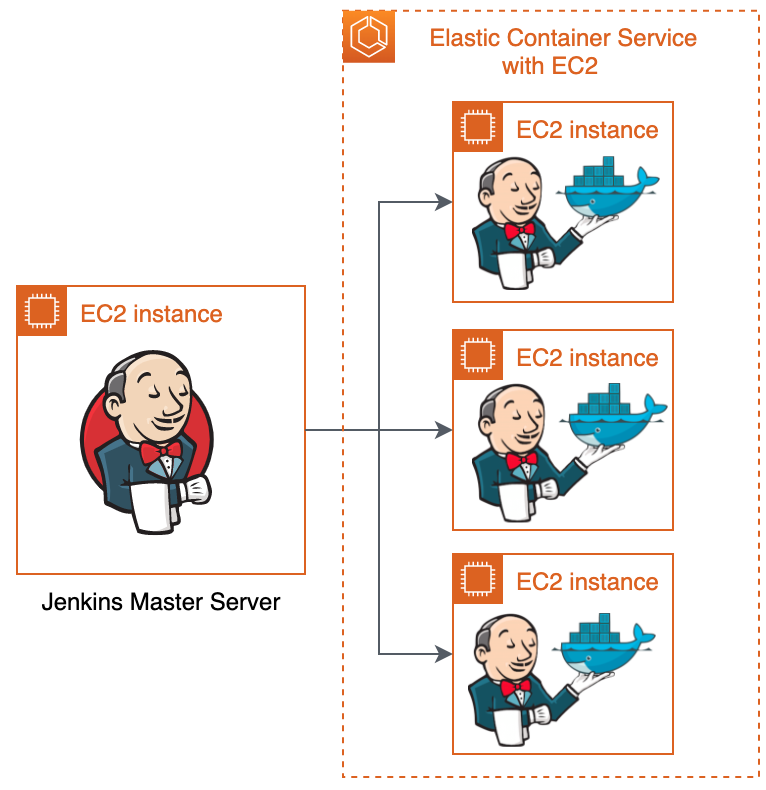
\includegraphics[width=\textwidth]{pics/jenkins-on-vm.png} % first figure itself
    \end{minipage}\hfill
    \begin{minipage}{0.54\textwidth}
        \centering
        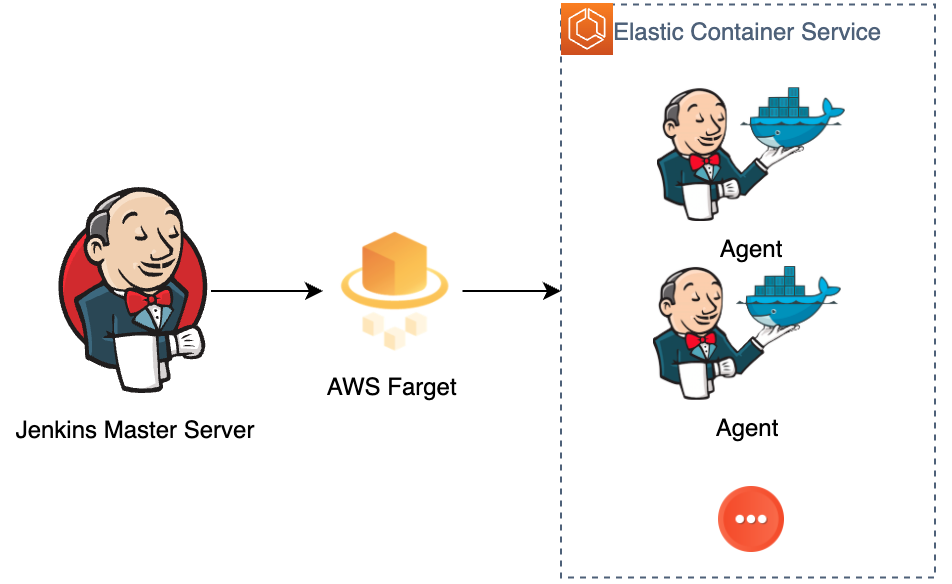
\includegraphics[width=\textwidth]{pics/jenkins-on-fargate.png} % second figure itself
    \end{minipage}
    \label{fig:ex1}
    \caption{Architecture diagram of the test Jenkins cluster with agents running in traditional virtual machines (left) and on ECS with AWS Fargate (right)}
\end{figure}
\subsubsection{Hardware}
The hardware of Jenkins agents is the independent variable that exposed to the change in the experiment.
\par
The experiments are conducted on Amazon Web Services (AWS). The hardware of Jenkins master node in both experiment groups is the same, which is EC2 instance of type t3.medium with 2 virtual CPU, 4 GB RAM and 30 GB disk. The EC2 instances as worker node is type t3.small, with 2 virtual CPU and 2GB RAM. Each worker has 2 Jenkins executer according to the Jenkins default setting. This means 2 containers could run in parallel on each EC2 virtual machine.
\par
In the control group, which is the implementation we presented in CH4, the Jenkins agents run on AWS ECS powered by AWS Fargate. The virtual hardware resources that are allocated to each serverless container is 1 virtual CPU, and 1 GB of RAM. This makes sure that each container shares the same hardware resources as in another group, so the hardware will not affect the result.
\subsubsection{Software}
We maintain the same software setup in each group. The operation System for EC2 instance that runs Jenkins master node is Ubuntu Server 18.04. The version of Jenkins that runs on the server is 2.222.3. For connect ECS and Fargate which works as the Jenkins agents, we use Jenkins plugin "Amazon Elastic Container Service (ECS) / Fargate", version 1.34. The container in Fargate/EC2 for running the Checkout and Build steps is from our developed docker image which you can find at \footnote{https://hub.docker.com/r/dry1995/jnlp}. The docker image includes essential dependencies that will be used to build the Spring Boot application and the base image which allow container connects Jenkins master as an agent. The "Build" step in our pipeline uses Gradle (version: 6.2.1) as the build tool for the application, the automated testing and code analysis is being integrated with this step, and being conducted by plugins of Gradle.

\par
To shows how does the 2 setups performance within the teams with different sizes, we run by run the different number of tasks parallel through the pipeline. This simulates the different team size, besides, it could also show the scalability when comes to the need for task parallelization in bigger organizations.

\subsection{Performance Properties and Evaluation}
We run the pipeline through 2 different setups, we will get the result of the following properties:
\begin{itemize}
    \item \textit{Runtime} describes the total time for finishing all the tasks.
    \item \textit{Cost Structure} describes the daily cost of 2 setups under the same workload, within the same period.
    \item \textit{Resource Utilization} describes the average CPU/RAM usage for each instance during a single run of the pipeline.
\end{itemize}
\subsection{Result}
//Here shows the result of the experiment
